% !TeX root = RJ-metapack-v1.tex
\title{\pkg{metapack}: An R Package for Bayesian Meta-Analysis and Network Meta-Analysis with a Unified Formula Interface}
\author{by Daeyoung Lim, Ming-Hui Chen, Joseph G. Ibrahim, Sungduk Kim, Arvind K. Shah and Jianxin Lin}

\maketitle

\abstract{
Meta-analysis, a statistical procedure that compares, combines, and synthesizes research findings from multiple studies in a principled
manner, has become popular in a variety of fields. Meta-analyses using study-level (or equivalently \emph{aggregate}) data are of particular interest due to data availability and modeling flexibility. In this paper, we describe an R package \pkg{metapack} that introduces a unified formula interface for both meta-analysis and network meta-analysis. The user interface---and therefore the package---allows flexible variance-covariance modeling for multivariate meta-analysis models and univariate network meta-analysis models. Complicated computing for these models has prevented their widespread adoption. The package also provides functions to generate relevant plots and perform statistical inferences like model assessments. Use cases are demonstrated using two real data sets contained in \pkg{metapack}.
}

\section{Introduction}\label{sec:intro}
The U.S. Food and Drug Administration provides a clear definition of meta-analysis as \emph{``the combining of evidence from relevant studies using appropriate statistical
methods to allow inference(s) to be made to the population of interest''} \citep{FDA2018metaanalysis}. In fields like medicine, pharmacology, and epidemiology, meta-analysis has become popular for reconciling conflicting results or corroborating consistent ones in multiple studies \citep{chalmers2002brief,borenstein2011introduction,hartung2011statistical,balduzzi2019perform}. Findings produced from meta-analyses are often placed at the apex of the evidence hierarchy \citep{FDA2018metaanalysis}.

R already has a large supply of meta-analysis packages. \CRANpkg{meta} \citep{meta2007} and \CRANpkg{rmeta} \citep{rmeta2018} use the method of moments
introduced in \citet{dersimonian1986meta}. \CRANpkg{metafor} \citep{metafor2010} further contains moderator analyses and fits meta-regression \citep{berkey1995random}
through weighted least squares. On the other hand, \CRANpkg{metaLik} \citep{metaLik2012} takes a likelihood approach based on the second-order approximation of the
modified likelihood ratio test statistic \citep{skovgaard1996explicit}. \CRANpkg{metatest} \citep{metatest2011} further includes hypothesis testing capabilities
through the likelihood ratio test with Barlett correction, and \CRANpkg{mvmeta} \citep{mvmeta2012} fits multivariate meta-analysis and meta-regression models via the
method of maximum likelihood. There are packages for Bayesian meta-analytic inference as well. \CRANpkg{bayesmeta} \citep{bayesmeta2020} assumes the normal-normal hierarchical random-effect model
and allows the user to choose prior distributions with a great deal of flexibility, both informative and noninformative. \CRANpkg{nmaINLA} \citep{nmaINLA2018} provides
functionalities for network meta-analysis and meta-regression with integrated nested Laplace approximations (INLA) as an alternative to the Markov chain
Monte Carlo (MCMC) algorithm. On the other hand, \CRANpkg{bmeta} \citep{bmeta2016} delivers flexible meta-analytic modeling by interfacing with JAGS
\citep{Plummer03jags:a}. {\color{black}\CRANpkg{MetaStan} \citep{MetaStan2020} provides binomial-normal hierarchical models with weakly informative priors, building upon the probabilistic language Stan \citep{RStan2020}.}

Despite its importance and the wide array of R packages available, meta-analysis is still regarded as a niche field that interests a narrow group of researchers and remains relatively low impact. We partially attribute this phenomenon to the fact that the R community has yet to come up with a user interface that unifies the theoretical distinctions between univariate and multivariate models, and between meta-analysis and network meta-analysis although the models have grown more complicated in the intervening years. Furthermore, a large class of simple Bayesian meta-analytic models is handled by probabilistic programming languages like Stan \citep{RStan2020} or BUGS \citep{R2OpenBUGS}. Meanwhile, many complex models are not easily programmable in probabilistic languages, and are not readily available in R. Especially, in the context of variance-covariance matrix modeling in (network) meta-analysis, \CRANpkg{metapack} is the first attempt in the R cosmos, to the best of our knowledge, to provide easy access to regression-modeling of the variances (of the treatment effects) as well as a wide array of options for modeling the response covariance matrices when the aggregate responses are multivariate with only a partially observed within-study sample covariance matrix.

\pkg{metapack} presented in this paper proposes a formula structure that flexibly represents the types of responses (univariate and multivariate) and the number of treatments (meta-analysis and network meta-analysis). The package also provides functions to assess model fits such as the deviance information criterion (DIC) and the logarithm of the pseudo-marginal likelihood (LPML), and to generate diagnostic plots. Some potential complications, theoretical and computational, in these model selection criteria may break the algorithm or erode the statistical inference when unaddressed (see Section~\nameref{subsec:model-comp}), which \pkg{metapack} takes care of by default---an advantage over model-agnostic programming languages.

The rest of this paper is organized as follows. {\color{black}Section~\nameref{sec:considered-models} briefly reviews the (network) meta-analysis model. Section~\nameref{sec:data-description} describes the general form of a meta-analysis data set to establish a generic data structure for meta-analysis and network meta-analysis. Section~\nameref{sec:basic-metapack} explains how the data structure can be represented using R's extended formula and how \pkg{metapack}'s main function parses it, and lays down the various modeling options for meta-analysis and network meta-analysis.} Section~\nameref{sec:performing-inference} further introduces the S3 methods available for performing statistical inferences and comparing models. Some computational considerations to accelerate the computation are detailed as well. Section~\nameref{sec:metapack-benchmark} provides demonstrations using the \emph{cholesterol} data and \emph{TNM} data included in \pkg{metapack}. Finally, Section~\nameref{sec:discussion} concludes the paper by offering a cautionary remark for multivariate meta-analysis models regarding the number of observations required to perform valid inferences on the correlation matrix, and discussing future research and package development directions.

\section{Considered models}\label{sec:considered-models}
In this section, we briefly review the models considered in \pkg{metapack}. There are largely two umbrella models: univariate or multivariate meta-analysis based on \cite{yao2015bayesian}, and univariate network meta-analysis based on \cite{li2021bayesian}. The various modeling options for each model introduced in this section \emph{encompass} the ones in \cite{yao2015bayesian} and \cite{li2021bayesian}. In what follows, the model description will deal with a general multivariate model including both meta-analysis and network meta-analysis, which is valid even when univariate response is assumed, i.e. $J=1$. Occasionally, the univariate model description will be provided side by side to avoid confusion.

Assume $K$ randomized controlled trials (RCTs) where the $k$-th trial includes $T_k$ treatment arms. Meta-analysis refers to a special case where $T_k=2$ for all $k=1,\ldots,K$. We adopt the notational abuse of omitting the trial indicator in the treatment's subscript. For instance, for the sample size of the $t$-th treatment arm of the $k$-th trial, we write $n_{kt}$, not $n_{t_kk}$. {\color{black}Furthermore, for readability, note that boldface lowercase Latin letters are vectors, while uppercase Latin letters are matrices. Boldface Greek letters can either be vectors or matrices and will be defined contextually.} Let $\bm{y}_{kt}$ be a $J$-dimensional aggregate response vector for the $t$-th treatment of the $k$-th trial. Similarly, let $\boldsymbol{x}_{ktj}\in \mathbf{R}^{p_j}$ be the treatment-within-trial level covariate corresponding to the $j$-th response, reflecting the fixed effects of the $t$-th treatment arm, and let $\boldsymbol{w}_{ktj} \in \mathbf{R}^{q_j}$ be the vector of covariates for the random effects. The model $\boldsymbol{y}_{kt}=\boldsymbol{X}_{kt}\boldsymbol{\beta} + \boldsymbol{W}_{kt} \boldsymbol{\gamma}_k + \boldsymbol{\epsilon}_{kt}$ describes the aggregate data model, where $\boldsymbol{\epsilon}_{kt} = (\epsilon_{kt1},\ldots,\epsilon_{ktJ})^\top$, $\boldsymbol{X}_{kt} = \oplus_{j=1}^J x_{ktj}^\top$ for which $\oplus$ indicates direct sum, $\boldsymbol{\beta} = (\boldsymbol{\beta}_1^\top,\ldots,\boldsymbol{\beta}_J^\top)^\top$, $\boldsymbol{W}_{kt}=\oplus_{j=1}^J \boldsymbol{w}_{ktj}^\top$, and $\boldsymbol{\gamma}_k = (\boldsymbol{\gamma}_{k1}^\top,\boldsymbol{\gamma}_{k2}^\top,\ldots,\boldsymbol{\gamma}_{kJ}^\top)^\top$. The aggregate (network) meta-analysis model becomes
\begin{equation}\label{eq:inital-mvmr}
\begin{dcases}
  \bm{y}_{kt} = \bm{X}_{kt}\bm{\beta} + \bm{W}_{kt} \bm{\gamma}_k + \bm{\epsilon}_{kt} \;\; \mbox{and} \;\; (n_{kt}-1)\bm{S}_{kt} \sim
  \mathcal{W}_{n_{kt}-1}(\Sigma_{kt}),&\text{if $J\geq 2$ (multivariate)}\\
  y_{kt} = \bm{x}_{kt}^\top\bm{\beta} + \bm{w}_{kt}^\top \bm{\gamma}_k + \epsilon_{kt} \;\; \mbox{and} \;\; (n_{kt}-1)s^2_{kt}/\sigma^2 \sim \chi^2_{n_{kt}-1},&\text{if $J=1$ (univariate)}
\end{dcases},
\end{equation}
 where $\bm{\epsilon}_{kt} \sim \mathcal{N}(\bm{0}, \Sigma_{kt}/n_{kt})$ or $\epsilon_{kt} \sim \mathcal{N}(0,\sigma_{kt}^2/n_{kt})$, $\bm{S}_{kt}$ is the sample covariance matrix, $s_{kt}^2$ is the sample variance, and $\Sigma_{kt} \in \mathcal{S}_{++}^J$ for which $\mathcal{S}_{++}^J$ is the space of $J\times J$ symmetric positive-definite matrices. In Equation \eqref{eq:inital-mvmr},  $\mathcal{W}_{\nu}(\Sigma)$ is the Wishart distribution
with $\nu$ degrees of freedom and a $J\times J$ scale matrix $\Sigma$ with density
\[
  p(X\mid \nu, \Sigma) = \dfrac{1}{2^{J\nu}|\Sigma|^{\nu/2}\Gamma_J(\nu/2)} |X|^{(\nu-J-1)/2}\exp\left(-\dfrac{1}{2}\mathrm{tr}(\Sigma^{-1}X) \right)I(X\in \mathcal{S}_{++}^J),
\]
where $\Gamma_J$ is the multivariate gamma function defined by \(\Gamma_J(z) = \pi^{J(J-1)/4}\prod_{j=1}^J \Gamma[z+(1-j)/2]\). $\chi_\nu^2$ indicates the chi-squared distribution with $\nu$ degrees of freedom. 

Stacking the random effects for all response endpoints, $\boldsymbol{\gamma}_k = (\boldsymbol{\gamma}_{k1}^\top, \ldots, \boldsymbol{\gamma}_{kJ}^\top)^\top$. Since the random effects are assumed to follow a distribution in the location-scale family (either a multivariate $t$-distribution or a multivariate normal distribution), i.e. $\boldsymbol{\gamma}_k \sim \mathcal{LS}(\boldsymbol{\gamma}, \Omega)$, the fixed-effect coefficient vector $\boldsymbol{\beta}$ absorbs the random effects' location parameter $\boldsymbol{\gamma}$, forming $\boldsymbol{\theta} = (\boldsymbol{\beta}^\top,\boldsymbol{\gamma}^\top)^\top$. The corresponding design matrix $\boldsymbol{X}_{kt}$ is also expanded to include the random-effect design matrix $\boldsymbol{W}_{kt}$, written as $\boldsymbol{X}_{kt}^* = [\boldsymbol{X}_{kt}, \boldsymbol{W}_{kt}]$. With $\boldsymbol{\gamma}_{k,o} = \boldsymbol{\gamma}_k - \boldsymbol{\gamma}$, the model now becomes
\begin{equation}\label{eq:model-centered}
  \begin{dcases}
    \bm{y}_{kt} = \bm{X}_{kt}^*\bm{\theta} + \bm{W}_{kt} \bm{\gamma}_{k,o} + \bm{\epsilon}_{kt},&\text{if $J\geq 2$ (multivariate)}\\
  \begin{split}
  y_{kt} &= {\bm{x}_{kt}^*}^\top\bm{\theta} + \bm{w}_{kt}^\top \bm{\gamma}_{k,o} + \epsilon_{kt}\\
    &\Rightarrow \boldsymbol{y}_k = \boldsymbol{X}_k^* \boldsymbol{\theta} + \boldsymbol{W}_k \boldsymbol{\gamma}_{k,o} + \boldsymbol{\epsilon}_k
  \end{split}
  ,&\text{if $J=1$ (univariate)}
  \end{dcases},
\end{equation}
where $\boldsymbol{y}_k=(y_{k,t_{k1}},\ldots,y_{k,t_{kT_k}})^\top$, $\boldsymbol{X}_k^*= ((\boldsymbol{x}^*_{k,t_{k1}})^\top,\ldots,(\boldsymbol{x}^*_{k,t_{kT_k}})^\top)^\top$, $\boldsymbol{W}_k = (\boldsymbol{w}_{k,t_{k1}}^\top,\ldots,\boldsymbol{w}_{k,t_{kT_k}}^\top)^\top$, and $\boldsymbol{\epsilon}_k=(\epsilon_{k,t_{k1}},\ldots,\epsilon_{k,t_{kT_k}})^\top$. We briefly restore the correct subscripts (i.e. $t_{kl}$ for $l=1,\ldots,T_k$) to demonstrate that $\boldsymbol{y}_k$, $\boldsymbol{X}_k^*$, and $\boldsymbol{W}_k$ may be different lengths and dimensions for different $k$'s. {\color{black}Here, $\{t_{k1},\ldots,t_{kT_k}\}$ denotes the set of treatments compared in the $k$-th trial.} The random effects are modeled differently in meta-analysis than in network meta-analysis. A major reason for this divergence is that the variables explaining the treatment effects are not easily found in the presence of varying numbers of treatments in different trials. The differences are further detailed in Section~\nameref{sec:mvma-model} and Section~\nameref{sec:network-meta}.

\section{Meta-analytic data for \pkg{metapack}}\label{sec:data-description}
To streamline configuring models in R formula, it is important to understand the data structure for \CRANpkg{metapack}. Table~\nameref{tab:data-structure} represents a typical {\color{black}arm-level data set for (network) meta-analysis, where each row represents a trial arm.} 
\begin{table}[H]
    \centering
    \resizebox{.98\linewidth}{!}{\begin{tabular}{ccccccc}\toprule
      \textbf{Outcome} ($\bm{y}_{kt}$) & \textbf{SD} ($s_{kt}$) & \textbf{DesignM1} ($\bm{x}_{kt}$) & \textbf{DesignM2} ($\bm{w}_{kt}$) & \textbf{Trial} (\code{k}) & \textbf{Treat} (\code{t}) & \textbf{n}\\\midrule
      $\bm{y}_{14}^\top$ & $s_{14}$ & $\bm{x}_{14}^\top$ & $\bm{w}_{14}^\top$ & 1 & 4 & 1000\\
      $\bm{y}_{11}^\top$ & $s_{11}$ & $\bm{x}_{11}^\top$ & $\bm{w}_{11}^\top$ & 1 & 1 & 545\\
      $\bm{y}_{21}^\top$ & $s_{21}$ & $\bm{x}_{21}^\top$ & $\bm{w}_{21}^\top$ & 2 & 1 & 1200\\
      $\vdots$ & $\vdots$ & $\vdots$ & $\vdots$ & $\vdots$ & $\vdots$ & $\vdots$\\ \bottomrule
    \end{tabular}}
  \caption{An example of arm-level meta-analytic data. {\color{black} \textbf{Trial} is equivalent to Study ID. A meta-analysis has two treatments in each trial for all trials, whereas a network meta-analysis can have trials with different numbers of treatments across trials. This distinction determines the number of rows for each trial (i.e. strictly two rows per trial in meta-analyses and a differing number of rows per trial for network meta-analyses). \code{Outcome}, \code{SD}, \code{DeisngM1}, and \code{DesignM2} can each be a vector, in which case the row vector representation indicates distributing across columns. For example, if \code{Outcome} consists of two endpoints, $(Y_1, Y_2)$, then each $\bm{y}_{kt}^\top$ should enter a row as two columns, \code{y1} and \code{y2}.}}
  \label{tab:data-structure}
\end{table}
\code{Outcome} is the response (or responses for multivariate cases), \code{SD} is the standard deviation(s) of the response(s), \code{DesignM1} and \code{DesignM2} are design matrices, and \code{n} is the arm sample size. The pair of trial and treatment indicators is unique to a row. {\color{black}The first design matrix, \code{DesignM1}, contains the covariates for fixed effects and will be written as $\bm{X}$ henceforth. The second design matrix, \code{DesignM2} or $\bm{W}$, represents different things depending on the model, which will be explained in Section~\nameref{sec:mvma-model} and Section~\nameref{sec:network-meta}. It should be noted that there can always be two design matrices, whose configuration will be illustrated in Section~\nameref{sec:basic-metapack}.}


A meta-analytic data set is characterized as folows: (1) univariate or multivariate and (2) meta-analysis or network meta-analysis. {\color{black}Here, meta-analysis refers to when trials have specifically two treatments (i.e. $t=1,2$ for all $k$) and all treatments are compared head to head. On the other hand, network meta-analysis includes more than two total treatments, where each trial can have a different set of treatments, allowing indirect comparison between treatments that are not compared head to head. The data structure is unchanged for network meta-analysis except that \code{Treat} can have more than two unique values.} The first category {\color{black}(univariate vs. multivariate)} is determined by the number of response endpoints, and the second category {\color{black}(meta- vs. network meta-analysis)} by the number of treatments. All other modeling choices fall into prior specification. 
\section{Basic implementation of \pkg{metapack}}\label{sec:basic-metapack}
\code{bmeta\_analyze} is the main function in \pkg{metapack}, whose first argument is an R formula. \code{bmeta\_analyze} internally parses a formula to identify a model and ultimately calls a \emph{worker function}. An extension of R's formula class, \CRANpkg{Formula} \citep{Formula}, accommodates multiple responses and parts, lending itself well into meta-analysis modeling. Once a model is fully identified, the MCMC algorithm is executed in C++, thanks to \CRANpkg{Rcpp} \citep{Rcpp2017} and \CRANpkg{RcppArmadillo} \citep{RcppArmadillo2014}. {\color{black}
\begin{table}[!htpb]
  \centering
  \resizebox{.99\linewidth}{!}{\begin{tabular}{lll}\toprule
    Name & Functionality & Description\\\midrule
    \code{bmeta\_analyze} & Estimation & Fits (network) meta-analysis models\\
    \code{hpd} & Inference & Computes highest posterior density (HPD) intervals of model parameters\\
    \code{model\_comp} & Inference & Computes model comparison measures (DIC or LPML)\\
    \code{print} &  & Displays a summary of the output\\
    \code{summary} & & Displays a summary of the output\\
    \code{plot} & & Plots trace plots, density plots, or surface-under-the-cumulative-ranking-curve (SUCRA) plots\\
    \code{fitted} & & Computes posterior means, standard deviations, and HPD intervals\\
    \code{coef} & & Computes posterior means of fixed-effect coefficients\\
    \code{cholesterol} & Data set & Cholesterol data for multivariate meta-analysis\\
    \code{TNM} & Data set & Triglyceride data for network meta-analysis\\\bottomrule
  \end{tabular}}
  \caption{A list of available functions and data sets in \CRANpkg{metapack}.}
\end{table}
}

\subsection{Using \code{Formula}}\label{subsec:using-formula}
The three characterizations of a meta-analytic data set must be encoded in the formula. Requiring the formula to have two left-hand sides (LHS) and two or three right-hand sides (RHS)\footnote{Semantically, the LHS should refer to the entire left of tilde---same for RHS---but in R idioms, when a side is counted or pluralized (e.g. LHSs, RHSs, or sides), it refers to a part or parts in the corresponding side.} is enough to communicate the characterizations for a wide class of meta-analysis models. We invite other R package developers to adopt the following representation for meta-analytic models, the general form of which is given by
\begin{example}
  y1 + y2 | sd1 + sd2 ~ x1 + x2 + x3 + ns(n) | w1 + w2 + w3 | treat + trial (+ groups)
\end{example}
Each \emph{part} in LHS or RHS is an R expression where variables (or functions of variables) are chained with a plus sign (\code{+})---e.g. \code{x1 + x2}. The tilde (\code{\textasciitilde}) separates all LHSs from all RHSs, each further separated into parts by vertical bars (\code{|}). The meaning of each part is syntactically determined by its location within the formula, like an English sentence. Therefore, every part must come in the exact order as prescribed for \code{bmeta\_analyze} to correctly identify the model.
\begin{itemize}
  \item The first LHS (\samp{y1 + y2}), the responses, is required of all models. Depending on the number of variables given in the first LHS, \code{bmeta\_analyze} will determine whether the model is multivariate or univariate. For example, a first LHS with only \code{y} would flag the model as univariate.
  \item The second LHS (\samp{sd1 + sd2}) supplies the standard deviations of the endpoints required of an aggregate-data meta-analysis. The function call will break if this part is missing.
  \item The first RHS (\samp{x1 + x2 + x3 + ns(n)}) defines the fixed-effect covariates. For aggregate-data models, the arm sample sizes must be passed as an argument to \code{ns()}. In the example code, \code{n} is the variable containing the arm sample sizes.
  \item The second RHS (\samp{w1 + w2 + w3}) defines either the random-effect covariates ($\boldsymbol{w}_{kt}^\top \boldsymbol{\gamma}$) or the variance-related covariates ($\log \tau_{kt} = \boldsymbol{w}_{kt}^\top \boldsymbol{\phi}$)---see {\color{black}Sections~\nameref{sec:mvma-model} or \nameref{sec:network-meta} for details}. This part is optional. If omitted, \code{bmeta\_analyze} will assume $\boldsymbol{w}_{kt}=\boldsymbol{1}$ where $\boldsymbol{1}$ is a vector of ones.
  \item The third RHS (\samp{treat + trial} or \samp{treat + trial + groups}) corresponds to the treatment and trial indicators, and optionally the grouping variable if it exists. Variables here must be provided in the exact order shown in the example.
\end{itemize}

The dimension of the response(s) is explicit in the formula, which determines the first characterization. The treatments are coerced to a factor---if not already one---whose number of levels is extracted (i.e. \samp{nlevels(treat)}) to resolve the second characterization, meta-analysis versus network meta-analysis.

\subsection{Function arguments}\label{subsec:function-arguments}
Aside from the first two arguments, \code{formula} and \code{data}, there are four other optional arguments that must be provided as R's \code{list} class: \code{prior}, \code{mcmc}, \code{control}, and \code{init}. All hyperparameters for the prior distributions should be included in \code{prior}---see Section~\nameref{sec:considered-models} for hyperparameters. \code{mcmc} only regards the numbers of MCMC iterations: \code{ndiscard} for the number of burn-in iterations, \code{nskip} for thinning, and \code{nkeep} for the posterior sample size. \code{control} configures the Metropolis-Hastings algorithm. \code{*\_stepsize} with the asterisk replaced with one of the parameter names indicates the step size for determining the sample evaluation points in the localized Metropolis algorithm. Lastly, initial values for the parameters can be provided in \code{init} in case a user has \emph{a priori} known high-quality starting points.



\subsection{Meta-analysis models}\label{sec:mvma-model}
For meta-analysis models, \pkg{metapack} acknowledges the possible existence of the first-line and second-line treatments trials. More generally, the trials may be grouped by a factor believed to generate disparate random effects. Although an arbitrary number of groups can exist in theory, we restrict our attention to two groups. Denoting the binary group indicators by $u_{kt}\in \{0,1\}$ yields
\begin{equation}\label{eq:meta-first-second-line}
  y_{ktj} = \bm{x}_{ktj}^\top \bm{\beta} + (1-u_{kt})\bm{w}_{ktj}^\top \bm{\gamma}_{kj}^0 + u_{kt}\bm{w}_{ktj}^\top \bm{\gamma}_{kj}^1 + \epsilon_{ktj}.
\end{equation}
The random effects are modeled as $\bm{\gamma}_{kj}^{l} \overset{\text{ind}}{\sim} \mathcal{N}({\bm{\gamma}_j^l}^*, \Omega_j^{l})$ and $(\Omega_j^{l})^{-1} \sim
\mathcal{W}_{d_{0j}}(\Omega_{0j})$. Stacking the vectors, $\bm{\gamma}_k^l = ((\bm{\gamma}_{k1}^l)^\top,\ldots,(\bm{\gamma}_{kJ}^l)^\top)^\top \sim
\mathcal{N}({\bm{\gamma}^l}^*,\Omega^l)$, where ${\bm{\gamma}^l}^* = (({\bm{\gamma}_1^l}^*)^\top,\ldots,({\bm{\gamma}_J^l}^*)^\top)^\top$, $\Omega_j =\Omega_j^0 \oplus \Omega_j^1$, and $\Omega = \oplus_{j=1}^J \Omega_j$ for $l\in \{0,1\}$. Adopting the \emph{noncentered parameterization} \citep{bernardo2003non}, define $\bm{\gamma}_{k,o}^l = \bm{\gamma}_k^l - {\bm{\gamma}^l}^*$. Denoting $\bm{W}_{kt}^* = [(1-u_{kt})\bm{W}_{kt},
u_{kt}\bm{W}_{kt}]$, $\bm{X}_{kt}^* = [\bm{X}_{kt}, \bm{W}_{kt}^*]$, $\bm{\theta} = (\bm{\beta}^\top,{{\bm{\gamma}^0}^*}^\top,
{{\bm{\gamma}^1}^*}^\top)^\top$, and $\bm{\gamma}_{k,o}
= ((\bm{\gamma}_{k,o}^0)^\top, (\bm{\gamma}_{k,o}^1)^\top)^\top$, the model is written as follows:
\begin{equation}\label{eq:final-mvmr}
  \bm{y}_{kt} = \bm{X}_{kt}^*\bm{\theta} + \bm{W}_{kt}^* \bm{\gamma}_{k,o} + \bm{\epsilon}_{kt}.
\end{equation}
If there is no distinction between the first-line and second-line therapies, then setting $u_{kt} = 0$ for all $(k,t)$ reduces the model back to Equation \eqref{eq:inital-mvmr}. Finally, we assume $\boldsymbol{\theta}\sim \mathcal{N}(\boldsymbol{0},c_0\boldsymbol{I})$ where $\boldsymbol{I}$ is an identity matrix.

A (boilerplate) template for this class of models is as follows:
\begin{example}
  f <- "y1 + y2 | sd1 + sd2 ~ x1 + x2 | w1 + w2 | treat + trial + groups"
  fit <- bmeta_analyze(formula(f), data = df,
          prior = list(c0 = [real], dj0 = [real], Omega0 = [matrix],
                       a0 = [real], b0 = [real],
                       d0 = [real], nu0 = [real], Sigma0 = [matrix]),
          control = list(sample_Rho = [logical], Rho_stepsize = [real],
                      R_stepsize = [real], delta_stepsize = [real], model = [string]))
\end{example}
We use \samp{real} and \samp{string} as aliases for \samp{double} and \samp{character} in R. Every bracketed expression should be replaced with an instance of the enclosed class. The hyperparameters in \samp{prior} and step sizes in \samp{control} will be clarified in the following modeling options. Note that all parameters with a step size are sampled through the Metropolis-Hastings algorithm.

\paragraph{Modeling options for $\Sigma_{kt}$} The covariance matrix between the response endpoints ($\Sigma_{kt}$) can be modeled depending on (1) the amount of data available; and (2) what assumptions the practitioner is willing to make. The diagonal elements of $\Sigma_{kt}$ are always identifiable whereas the off-diagonal elements require additional modeling assumptions. \pkg{metapack} presently offers five options, specifiable through \code{model} in the \code{control} argument. For $\mathcal{M}_2$--$\mathcal{M}_5$, the unobserved sample correlation matrices are sampled from their conditional distributions $(R_{kt}\mid V_{kt},\Sigma_{kt})$ given by
\begin{equation}\label{eq:sample-correlation-density}
  p(R_{kt}\mid V_{kt},\Sigma_{kt}) \propto |R_{kt}|^{(n_{kt}-J-2)/2} \exp\left\{-\dfrac{(n_{kt}-1)}{2}\mathrm{tr}\left(V_{kt}^{\frac{1}{2}}\Sigma_{kt}^{-1}V_{kt}^{\frac{1}{2}}R_{kt} \right) \right\}.
\end{equation}
\begin{itemize}
  \item ($\mathcal{M}_1$: \code{model="NoRecovery"}) The simplest and easiest way to model the covariance matrices is to relinquish correlation recovery, in which case Equation~\eqref{eq:sample-correlation-density} is ignored. We assume $\Sigma_{kt} = \mathrm{diag}(\sigma_{kt,11}^2,\ldots, \sigma_{kt,JJ}^2)$ with $\sigma_{kt,jj}^2 \sim \mathcal{IG}(a_0,b_0)$ for $a_0,b_0>0$, where $\mathcal{IG}(a,b)$ denotes the
inverse-gamma distribution whose density function is proportional to $x^{-(a+1)} \exp(-b/x)$ for $x>0$. For univariate meta-analyses, this is the only valid option since there are no off-diagonal entries.

\item ($\mathcal{M}_2$: \code{model="EquiCovariance"}) We can assume the covariance matrix is for all pairs of treatments and trials. That is, $\Sigma_{kt} = \Sigma$ for every combination of $(k,t)$ for $t=1,\ldots,T$ and
$k=1,\ldots,K$. A Wishart prior distribution is assumed for $\Sigma^{-1}$, i.e. $\Sigma^{-1} \sim \mathcal{W}_{s_0}(\Sigma_0)$ for $s_0>J-1$ and $\Sigma_0\in \mathcal{S}_{++}^J$.


\item ($\mathcal{M}_3$: \code{model="EquiWithinTreat"}) If the equal covariance is too strong an assumption, we can allow the covariance matrices to be equivalent within a treatment. That is,
$\Sigma_{kt} = \Sigma_t$ for $t=1,\ldots,T$. Similar to $\mathcal{M}_2$, a Wishart prior distribution is assumed for $\Sigma_t^{-1}$, i.e. $\Sigma_t^{-1} \sim \mathcal{W}_{s_0}(\Sigma_0)$.


\item ($\mathcal{M}_4$: \code{model="EquiCorrelation"}) To achieve the best of both worlds---variances and correlations---we can let the variances enjoy maximum freedom but attempt to recover the correlations by restricting them to be identical across treatments and trials for identifiability. Performing the decomposition,
$$
\Sigma_{kt} = \bm{\delta}_{kt}\bm{\rho} \bm{\delta}_{kt},
$$
where $\bm{\delta}_{kt} = \mathrm{diag}(\Sigma_{kt,11}^{1/2},\ldots,\Sigma_{kt,JJ}^{1/2})$, and $\bm{\rho}$ is the correlation matrix, the elements in $\bm{\delta}_{kt}$ and $\bm{\rho}$ are sampled through the Metropolis-Hastings algorithm.


\item ($\mathcal{M}_5$: \code{model="Hierarchical"}) The hierarchical prior for $\Sigma_{kt}$ is given by $(\Sigma_{kt}^{-1}\mid \Sigma) \sim \mathcal{W}_{\nu_0}((\nu_0-J-1)^{-1}\Sigma^{-1})$ and $\Sigma \sim \mathcal{W}_{d_0}(\Sigma_0)$. By allowing the $\Sigma_{kt}$'s to differ but having them share information across treatments and trials via $\Sigma$, this assumption aims to control the between-treatment and between-trial variations simultaneously. Since the amount of information shared between treatments and trials is controlled by $\nu_0$ $(>J-1)$, it is advised to try multiple values for $\nu_0$ and perform a model assessment through the deviance information criterion (DIC) or the logarithm of the pseudo-marginal likelihood (LPML). $\Sigma$ is further decomposed for Metropolis-Hastings algorithm as $\Sigma=\Delta \boldsymbol{\rho}\Delta$ where $\Delta = \mathrm{diag}(\delta_1,\ldots,\delta_J)$ is the diagonal matrix of standard deviations, and $\boldsymbol{\rho}$ is a correlation matrix with unit diagonal elements. 


\end{itemize}

\subsection{Network meta-analysis models}\label{sec:network-meta}
For univariate network meta-analysis, {\color{black}the design matrix for random effects} is restricted to be the selection matrix $E_k^\top = (e_{t_{k1}}, e_{t_{k2}}, \ldots, e_{t_{k T_k}})^\top$, where $e_{t_{kl}}=(0,\ldots, 1,\ldots,0)^\top$,
$l=1,\ldots,T_k$, with the $t_{kl}$th element set to 1 and 0 otherwise, and $T_k$ is the number of treatments included in the $k$-th trial. Furthermore, we redefine $\boldsymbol{\gamma}_{k,o}$ to be $\boldsymbol{\gamma}_{k,o}:= E_k^\top \boldsymbol{\gamma}_k$, a vector of $T_k$-dimensional scaled random effects. The random effects $\boldsymbol{\gamma}_k \sim t_T(\boldsymbol{\gamma},\boldsymbol{\rho},\nu)$, where $t_T(\boldsymbol{\mu},\Sigma,\nu)$ denotes a multivariate $t$-distribution with $\nu$ degrees of freedom, a location parameter vector $\boldsymbol{\mu}$, and a scale matrix $\Sigma$. $T$ indicates the number of distinct treatments in all trials. The random effects $\boldsymbol{\gamma}_k$ are scaled since $\boldsymbol{\rho}$ is a correlation matrix with unit diagonal entries, and the variance components can be modeled as a multiplicative term. That is, with $\bm{W}_k(\bm{\phi}) = \mathrm{diag}(\exp(\bm{w}_{kt_{k1}}^\top \bm{\phi}), \ldots, \exp(\bm{w}_{kt_{k T_{k}}}^\top \bm{\phi}))$, the model is recast as
\[
  \bm{y}_{k} = \bm{X}_k^*\bm{\theta} + \bm{W}_k(\bm{\phi})\bm{\gamma}_{k,o} + \bm{\epsilon}_k,
\]
where $\bm{X}_k^* = (\bm{X}_k, E_k^\top)$, $\bm{\theta} = (\bm{\beta}^\top, \bm{\gamma}^\top)^\top$, $\bm{\epsilon}_k \sim
\mathcal{N}_{T_k}(\bm{0},\Sigma_k)$, and $\Sigma_k = \mathrm{diag}\left(\frac{\sigma_{kt_{k1}}^2}{n_{kt_{k1}}}, \ldots, \frac{\sigma_{kt_{k T_{k}}}^2}{n_{kt_{k
T_{k}}}}\right)$. This allows $\exp(\boldsymbol{w}_{kt}^\top \boldsymbol{\phi})$ to be the standard deviation of $\gamma_{kt}$. Since the multivariate $t$-random effects are not analytically marginalizable, we represent it as a scale mixture of normals as
\begin{equation}\label{eq:nma-hierarchical-re}
  (\bm{\gamma}_{k,o}\mid \lambda_k) \overset{\text{ind}}{\sim}\mathcal{N}_{T_k}
  \left(\bm{0},\lambda_k^{-1}(E_k^\top \bm{\rho}E_k) \right),\qquad \lambda_k \overset{\text{iid}}{\sim}\mathcal{G}a\left(\frac{\nu}{2},\frac{\nu}{2} \right),
\end{equation}
where $\mathcal{G}a(a,b)$ indicates the gamma distribution with mean $a/b$. Finally, $\boldsymbol{\theta} \sim \mathcal{N}(\boldsymbol{0},c_{01}\boldsymbol{I})$ and $\boldsymbol{\phi} \sim \mathcal{N}(\boldsymbol{0},c_{02}\boldsymbol{I})$.

A (boilerplate) template for this class of models is as follows:
\begin{example}
  f <- "y | sd ~ x1 + x2 | w1 + w2 | treat + trial"
  fit <- bmeta_analyze(formula(f), data = df,
            prior = list(c01 = [real], c02 = [real], df = [real],
              a4 = [real], b4 = [real], a5 = [real], b5 = [real]),
            control = list(sample_df = [logical], sample_Rho = [logical],
              Rho_stepsize = [real], phi_stepsize = [real], lambda_stepsize = [real]))
\end{example}
Every bracketed expression should be replaced with an instance of the enclosed class. The hyperparameters in \samp{prior} and step sizes in \samp{control} will be clarified in the following modeling options. Note that all parameters with a step size are sampled through the Metropolis-Hastings algorithm.

\paragraph{Modeling options} The appeal of considering heavy-tailed random effects and modeling the variance to be a deterministic linear function of a covariate is that both extend but still cover the common cases (normal random effects and no variance modeling) as either the limiting or a special case. Unlike meta-analysis, there is no single argument (\samp{model}) determining the modeling option. A model is rather specified by a combination of arguments.
\begin{itemize}
  \item ($\mathcal{M}_1$ - No variance modeling) Sometimes, no covariate information is available for modeling the variances, where $\boldsymbol{w}_{kt_{kt}}$ reduces to one---$\boldsymbol{W}_k(\boldsymbol{\phi}) = \mathrm{diag}(\mathrm{e}^\phi,\ldots,\mathrm{e}^\phi)$. The marginal variance of $y_{kt}$ becomes $\mathrm{Var}(y_{kt})=\sigma_{kt}^2/n_{kt}+\mathrm{e}^{2\phi}$. This can be achieved by simply omitting the \emph{second RHS}, thereby making the trial and treatment configuration the second RHS. For example, \samp{y | sd \textasciitilde  x1 + x2 | treat + trial}.
  \item ($\mathcal{M}_2$ - Normal random effects) In the limiting case where $\nu\to\infty$, $\bm{\gamma}_{k,o} \sim \mathcal{N}_{T_k}(0,E_k^\top \boldsymbol{\rho}E_k)$. \code{bmeta\_analyze} treats $\nu$ (\samp{df}) as part of the prior specification. Thus, \samp{df=Inf} in the \samp{prior} argument corresponds to opting for normal random effects.
  \item ($\mathcal{M}_3$ - Random degrees of freedom) The degrees of freedom of the multivariate $t$-distribution for the random effects are treated as unknown. In this case, a hierarchical prior is considered for the degrees of freedom. That is, $(\nu\mid \nu_a,\nu_b) \sim \mathcal{G}a(\nu_a,\nu_a/\nu_b)$, $\nu_a \sim \mathcal{G}a(a_4,b_4)$, and $\nu_b \sim \mathcal{IG}(a_5,b_5)$. Since sampling $\nu$ regards the MCMC algorithm, a logical variable \samp{sample\_df} is placed in the \samp{control} argument. If \samp{sample\_df=TRUE}, the value for \samp{df} in \samp{prior} will be used as the initial value, and the related hyperparameters (\samp{a4}, \samp{b4}, \samp{a5}, and \samp{b5}) can be set in \samp{prior}. For obvious reasons, \samp{df} cannot be assigned \samp{Inf} if \samp{sample\_df=TRUE}.
\end{itemize}


\section{Performing inference}\label{sec:performing-inference}
The object (\code{fit}) returned from \code{bmeta\_analyze} remembers the function arguments, encapsulates the model specification, and contains the posterior sample from the MCMC algorithm. Therefore, this object alone can be passed to other methods to perform subsequent inferences. These methods include \code{fitted}, \code{hpd}, \code{coef}, \code{model\_comp}, and \code{sucra}.

The posterior means, standard deviations, and the HPD intervals are computed via the \code{fitted()} function. The \code{fitted()} function has two optional arguments: \samp{level} and \samp{HPD}. \samp{level} determines the credibility level of the interval estimation. \samp{HPD}, a logical parameter, decides whether a highest posterior density or equal-tailed credible interval will be produced. It is also possible to obtain the posterior interval estimates only using \code{hpd()}.
\begin{example}
R> est <- fitted(fit, level=0.99, HPD = TRUE)
R> hpd <- hpd(fit, level = 0.95, HPD = TRUE)
\end{example}
\samp{coef(fit)} allows users to extract the posterior mean of the fixed-effect coefficients.

\paragraph{Model comparison}\label{subsec:model-comp}
It is crucial to determine a suitable model to base the statistical inference on. Section~\nameref{sec:mvma-model} introduces five models for $\Sigma_{kt}$, and Section~\nameref{sec:network-meta} contains infinitely many models since the degrees of freedom $\nu$ for the random effects can assume any number on the positive real line including infinity. Such a circumstance calls for a principled way of comparing models as well as evaluating goodness of fit.

The deviance information criterion \citep{spiegelhalter2002bayesian}, or DIC, is defined as follows:
\[
  \mathrm{DIC} = \mathrm{Dev}(\bar{\bm{\eta}}) +2 p_D,
\]
where $\bm{\eta}$ indicates all model parameters for which $\bar{\bm{\eta}} = \mathbb{E}[\bm{\eta}\mid D_{\text{obs}}]$. $\mathrm{Dev}(\bm{\eta})$ is the deviance function given by $\mathrm{Dev}(\bm{\eta}) = -2 \log L_{o\mathbf{y}}(\bm{\eta}\mid D_{\text{obs}})$, for which $L_{o\mathbf{y}}$ is the observed-data likelihood associated with $\bm{y}$, and $p_D$ is defined as $p_D = \overline{\mathrm{Dev}(\bm{\eta})} -\mathrm{Dev}(\bar{\bm{\eta}})$ where $\overline{\mathrm{Dev}(\bm{\eta})} =\mathbb{E}[\mathrm{Dev}(\bm{\eta})\mid D_{\text{obs}}]$.
\begin{example}
R> dic <- model_comp(fit, type = "dic", verbose = TRUE, ncores = 3)
\end{example}

Another Bayesian model selection criterion is the logarithm of the pseudo-marginal likelihood (LPML), defined as the summed logarithm of the conditional predictive ordinates (CPO). The CPO has a ``leave-one-out'' predictive interpretation, which in meta-analyses is often overlooked---a significant oversight that will undermine model comparison. The aggregate nature of meta-analysis data calls for a redefinition of what is ``left out'' and what should be the base unit for prediction. With trials as the base unit, the CPO for the $k$-th trial is
\[
  \mathrm{CPO}_k = \int L(\bm{\eta}\mid D_{o\mathbf{y}})p(\bm{\eta}\mid D_{o\mathbf{y}}^{-k},D_{o\mathbf{s}})\,\mathrm{d}\bm{\eta},
\]
where $D_{o\mathbf{y}}^{-k}$ is $D_{o\mathbf{y}}$ with the $k$-th trial removed, and $p(\bm{\eta}\mid D_{o\mathbf{y}}^{-k},D_{o\mathbf{s}})$ is the posterior distribution based on the data without the $k$-th trial. Then, $\mathrm{LPML} = \frac{1}{K}\sum_{k=1}^K \log (\mathrm{CPO}_k)$.
\begin{example}
R> lpml <- model_comp(fit, type = "lpml", verbose = TRUE, ncores = 3)
\end{example}
Treatments included in only one trial violate the predictive interpretation of the CPO. The corresponding trials thus should be removed from LPML calculation. \code{model\_comp} returns the logarithm of the CPO of every trial but corrects the LPML should such treatments exist. For those occasions, a naive sum of the logarithm of the $\mathrm{CPO}_k$'s will not equal the corrected LPML in the returned object.

The DIC and LPML for the meta-analysis models are relatively straightforward since the observed-data likelihood is a multivariate normal density. However, network meta-analysis models require some technical considerations in evaluating the following observed-data likelihood that involves an analytically intractable integral when $t$-random effects are used: slow computation speed and numerical overflow. Observe the following observed likelihood function for the network meta-analysis model:
\begin{align*}
  L_{o\mathbf{y}}(\bm{\eta}\mid D_\text{obs}) = \prod_{k=1}^K \int_0^\infty &(2\pi)^{-\frac{T_k}{2}}g(\lambda_k)\left| \lambda_k^{-1}(\bm{W}_k(\bm{\phi})E_k^\top\bm{\rho}E_k \bm{W}_k(\bm{\phi})) + \Sigma_k \right|^{-\frac{1}{2}}\\
    &\times \exp\left\{-\dfrac{(\bm{y}_k - \bm{X}_k^*\bm{\theta})^\top\left[\lambda_k^{-1}\bm{W}_k(\bm{\phi})E_k^\top \bm{\rho}E_k \bm{W}_k(\bm{\phi})+\Sigma_k \right]^{-1}(\bm{y}_k - \bm{X}_k^*\bm{\theta})}{2}\right\}\,\mathrm{d}\lambda_k,
\end{align*}
where $g(\lambda_k)$ is the gamma density with shape and rate parameters $\nu/2$.
The integral is evaluated via double exponential (DE) quadrature, or equivalently tanh-sinh quadrature \citep{takahasi1974double,Bailey2005}, available in the \pkg{math} header of the \CRANpkg{BH} package \citep{BHboost2019}. DE quadrature is robust to singularities, terminates fast, and provides high precision \citep{Bailey2005}. We address the slow speed through \emph{``shared memory multiprocessing programming''} via \pkg{OpenMP} \citep{openmp18}. \pkg{OpenMP} is a widely used application programming interface (API) for portable and scalable parallel processing in {C}, {C++}, and {Fortran} across many operating systems. As long as R is configured for \pkg{OpenMP}, \pkg{metapack} will deploy parallelism. Unless the argument \code{ncores} is specified otherwise, \code{model\_comp} will use two CPU cores for parallel computing by default.

To prevent overflow, we take the following steps:
\begin{itemize}
   \item Let $h(\lambda_k)$ denote the integrand. Then, compute \(\widehat{\lambda}_k = \arg\max_{\lambda_k} \log h(\lambda_k)\).
   \item Redefine the integral as
   \[
    \exp\left\{\log h(\widehat{\lambda}_k) + \log \int_0^\infty\exp\left[\log h(\lambda_k) - \log h(\widehat{\lambda}_k) \right]\,\mathrm{d}\lambda_k\right\}.
   \]
 \end{itemize}
 Although the exponential shifting scheme does not warrant preventing every occurrence of numerical overflow, we have observed stable evaluations of the integral for over several thousand batches of simulations.


\subsection[Model diagnostics and visualization]{Model diagnostics and visualization}\label{subsec:model-diag}
It is important to diagnose whether the results are consistent with the assumptions and visualize the findings. \pkg{metapack} provides methods for these: \code{plot} and \code{sucra}. The \code{plot} method is available for both meta-analysis and network meta-analysis whereas \code{sucra} is exclusively for network meta-analysis.

The \code{plot} method will take the \code{fit} object and generate the density plots and trace plots of $\bm{\theta}$. To see the plots for other parameters, run the following commands using \CRANpkg{coda} \citep{coda2006}:
\begin{example}
R> library("coda")
R> posterior <- as.mcmc(data.frame(gammaR = fit$mcmc.draws$gamR,
+    sig2 = fit$mcmc.draws$sig2))
R> plot(posterior)
\end{example}
Similarly, \CRANpkg{boa} \citep{BOA2007} can be used for output analysis. The posterior sample of $\bm{\rho}$ comes in three-dimensional arrays, which requires suitable indexing to generate trace plots for the off-diagonal lower-triangular elements. To generate such trace plots, run the following command:
\begin{example}
R> idx <- lower.tri(fit$mcmc.draws$Rho[,,1])
R> n_idx <- ncol(idx) * (ncol(idx) - 1) / 2
R> posterior <- as.mcmc(data.frame(
+                 rho = t(vapply(1:fit$mcmc$nkeep, function(ikeep) {
+                   rho_i <- fit$mcmc.draws$Rho[,,ikeep]
+                   rho_i[idx]
+                 }, FUN.VALUE=numeric(n_idx)))))
R> plot(posterior)
\end{example}

\paragraph{Treatment comparisons}\label{subsec:treatment-comp} The \emph{surface under the cumulative ranking (SUCRA)} curve is useful when the ranking of the treatments in a network meta-analysis is of interest. Based on the
posterior sample, $\mathbb{P}(t,r)$ denotes the probability that the treatment $t$ is ranked $1\leq r \leq T$ for $t=1,\ldots,T$. Let $\mathbf{P}$ be the $T\times
T$ discrete rank (row-stochastic) probability matrix whose $(t,r)$th element is $\mathbb{P}(t,r)$. The cumulative probability is then computed through \(F(t,x) = \sum_{r=1}^x \mathbb{P}(t,r),\)
where $F(t,x)$ is the probability that the $t$-th treatment is ranked $x$ or better. Since $F(t,T)=1$ for every $t$, the surface under
the cumulative ranking distribution for the $t$-th distribution is given by
\[
  \mathrm{SUCRA}(t) = \dfrac{1}{T-1}\sum_{x=1}^{T-1}F(t,x).
\]
\code{sucra} will take the \code{fit} object and return the SUCRA and the discrete rank probability matrix $\mathbf{P}$.
\begin{example}
R> s <- sucra(fit)
R> s$SUCRA
R> s$rankprob
\end{example}
If only plotting is needed, the storage of the \code{sucra} object can be bypassed via running \code{plot(sucra(fit))}. Note
that SUCRA $s$ has a bijection with the mean rank $r$ of a treatment, $r = 1 + (1-s)(T-1)$, where $T$ is the number of treatments.


\section{Demonstration with real data}\label{sec:metapack-benchmark}
\subsection{Meta-analysis}\label{subsec:benchmark-mvmr}
\pkg{metapack} includes a data set, \code{cholesterol}, which consists of 26 double-blind, randomized, active, or placebo-controlled clinical trials on patients with primary hypercholesterolemia sponsored by Merck \& Co., Inc., Kenilworth, NJ, USA \citep{yao2015bayesian}. The data set can be loaded by running \code{data("cholesterol")}. The \code{cholesterol} data set has three endpoints: low density lipoprotein cholesterol (\code{pldlc}), high density lipoprotein cholesterol (\code{phdlc}), and triglycerides (\code{ptg}). The percent change from the baseline in the endpoints, variables prefixed by \code{p-}, are the aggregate responses, followed by the corresponding standard deviations prefixed by \code{sd-}.
\begin{table}[!htbp]
\centering
\begin{tabular}{ll}\toprule
Variable & Description \\ \midrule
\code{study} & study identifier\\
\code{trial} & trial identifier\\
\code{treat} & treatment indicator for Statin or Statin+Ezetimibe\\
\code{n} & the number of participants in the study arms\\
\code{pldlc} & aggregate percentage change in LDL-C\\
\code{phdlc} & aggregate percentage change from baseline in HDL-C\\
\code{ptg} & aggregate percentage change from baseline in triglycerides (TG)\\
\code{sdldl} & sample standard deviation of percentage change in LDL-C\\
\code{sdhdl} & sample standard deviation of percentage change in HDL-C\\
\code{sdtg} & sample standard deviation of percentage change in triglycerides (TG)\\
\code{onstat} & whether the participants were on Statin prior to the trial\\
\code{bldlc} & baseline LDL-C\\
\code{bhdlc} & baseline HDL-C\\
\code{btg} & baseline triglycerides (TG)\\
\code{age} & age in years\\
\code{white} & the proportion of white participants\\
\code{male} & the proportion of male participants\\
\code{dm} & the proportion of participants with diabetes mellitus\\
\code{durat} & duration in weeks\\\bottomrule
\end{tabular}
\caption{Variables included in the \code{cholesterol} data set.}\label{tab:cholesterol-variables}
\end{table}
Variable documentation is also available in \code{help("cholesterol")}.

\begin{example}
R> set.seed(2797542)
R> f_1 <- 'pldlc + phdlc + ptg | sdldl + sdhdl + sdtg ~ 
+    0 + bldlc + bhdlc + btg + age + durat + white + male + dm + ns(n) | treat |
+    treat + trial + onstat'
R> fit_ma <- bmeta_analyze(formula(f_1), data = cholesterol,
+   prior = list(model="NoRecovery"),
+   mcmc = list(ndiscard = 1000, nkeep = 1000),
+   control=list(scale_x = TRUE, verbose=TRUE))
\end{example}


\begin{figure}[H]
  \centering
  \includegraphics[scale=0.7]{ma_traceplots.eps}
  \caption{The trace plots (three top panels) and density plots (three bottom panels) of the treatment effects from the meta-analysis model generated from \code{plot(fit\_ma)}---plots have been omitted for brevity. The trace plots show good mixing and convergence of MCMC chains and the density plots indicate that the marginal posterior distribution for each treatment effect is roughly symmetric. The MCMC samples of the regression coefficients will be automatically assigned row names according to the formula provided by the user. \samp{treat*(1-2nd)\_3} indicates the treatment effect within the first-line patients (i.e. \samp{onstat=0}) with respect to the third response variable, \samp{ptg}. Likewise, \samp{(Intercept)*2nd\_3} is the baseline effect within the second-line patients (i.e. \samp{onstat=1}) with respect to \samp{ptg}.}
  \label{fig:traceplot-mvmr}
\end{figure}

\code{summary} can be used to summarize the posterior sample from the \samp{fit} object. \code{summary} will name the variables accordingly in the output, suffixed by the index $j$ in the corresonding outcome variable $y_{ktj}$. For example, \samp{bldlc\_1} in the output below corresponds to the base LDL-C's coefficient associated with the first endpoint (\samp{pldlc}). The summary table consists of the posterior mean, posterior standard deviation, the HPD lower bound, and the HPD upper bound. Users may choose to compute the equal-tailed credible intervals (CI) instead of the HPD intervals by setting \samp{HPD=FALSE}.
\begin{example}
R> summary(fit_ma, HPD = TRUE, level = 0.95)
Call:
bmeta_analyze(formula = formula(f_1), data = cholesterol,
  prior = list(model = "NoRecovery"), 
  mcmc = list(ndiscard = 1000, nkeep = 1000), control = list(scale_x = TRUE, 
        verbose = TRUE))
Fixed-effects:
                       Post.Mean  Std.Dev  HPD(Lower)  HPD(Upper)
bldlc_1                   0.1394   0.0938     -0.0532      0.3051
bhdlc_1                  -0.5146   0.6329     -1.7641      0.7243
btg_1                     0.0018   0.0818     -0.1693      0.1607
age_1                     0.3785   0.4389     -0.5308      1.1648
durat_1                   0.9699   0.5234     -0.1658      1.9979
white_1                  -5.2449   7.4048    -19.7345      8.9764
male_1                   -1.2652  12.3948    -25.6807     23.0538
dm_1                      0.3987   5.3392    -10.4995      9.4673
bldlc_2                  -0.0128   0.0137     -0.0393      0.0134
bhdlc_2                  -0.0294   0.1280     -0.2887      0.2149
btg_2                     0.0228   0.0212     -0.0203      0.0619
age_2                    -0.0963   0.0735     -0.2422      0.0460
durat_2                  -0.0007   0.0712     -0.1320      0.1382
white_2                   5.5822   1.3044      3.0802      8.1901
male_2                   -2.1449   2.6956     -7.5975      2.6164
dm_2                     -1.0457   1.0923     -3.1816      1.0341
bldlc_3                   0.0141   0.0406     -0.0719      0.0853
bhdlc_3                   0.0082   0.2637     -0.5278      0.4872
btg_3                    -0.0734   0.0467     -0.1598      0.0154
age_3                    -0.1385   0.2043     -0.5077      0.2591
durat_3                   0.0996   0.2546     -0.3718      0.6080
white_3                  -0.7053   5.2345    -11.0570      8.9591
male_3                   14.5482   7.1735      0.0642     28.2959
dm_3                      5.0535   2.9542     -1.4157     10.5545
(Intercept)*(1-2nd)_1   -42.8675   3.2934    -48.8356    -35.8794
treat*(1-2nd)_1         -12.1435   1.1211    -14.4040    -10.0135
(Intercept)*2nd_1        -3.2219   3.0426     -9.3109      2.7419
treat*2nd_1             -20.0843   1.5235    -23.3169    -17.2637
(Intercept)*(1-2nd)_2     5.1425   0.5840      3.8240      6.1036
treat*(1-2nd)_2           2.0787   0.4718      1.0663      3.0222
(Intercept)*2nd_2         0.7346   0.5814     -0.3377      1.8738
treat*2nd_2               1.3482   0.3116      0.7579      1.9880
(Intercept)*(1-2nd)_3   -18.5035   2.1543    -22.3232    -13.7985
treat*(1-2nd)_3          -4.7726   0.9952     -6.7784     -2.9511
(Intercept)*2nd_3        -4.1805   1.2910     -6.7672     -1.7005
treat*2nd_3              -8.8579   0.9443    -10.6208     -7.0530
---------------------------------------------------
*HPD level:  0.95 
\end{example}
  {\color{black} The suffixed \samp{\_j} where \texttt{j} can be 1, 2, or 3 corresponds to the response endpoint. Since \code{scale\_x = TRUE} is equivalent to \code{scale(<var>, center=TRUE, scale=TRUE)}, the covariates have been centered, which affects the interpretation of the intercepts. This allows us to interpret \code{(Intercept*(1-2nd)\_1)=-42.8675} as the statin effect in the first-line studies, where \code{2nd} represents the indicator variable for second-line studies evaluating to one if second-line and zero otherwise. On the other hand, the coefficient estimate -12.1435 for \code{treat*(1-2nd)\_1} is the Statin+Ezetimibe effect, compared to administering statin alone. For the second-line studies where patients had already been on statin, \code{(Intercept)*2nd\_1=-3.2219} came out insignificant, according to the 95\% HPD interval, as anticipated because the treatment for this group was merely a continuation of taking statin. The coefficient estimate -20.0843 for \code{treat*2nd\_1} shows that ezetimibe on top of statin has a greater cholesterol-lowering effect than statin alone.}

\code{print} is similar to \code{summary} but additionally prints the model specification. The output from \samp{print(fit\_ma)} is given as follows.
\begin{example}
R> print(fit_ma, HPD = TRUE, level = 0.95)
Call:
bmeta_analyze(formula = formula(f_1),
    data = cholesterol, prior = list(model = "NoRecovery"),
    mcmc = list(ndiscard = 1000, nkeep = 1000),
    control = list(scale_x = TRUE, verbose = TRUE))
Model:
  (Aggregate mean)
    y_kt = X_kt * theta + W_kt * gamma_k + N(0, Sigma_kt / n_kt)
  (Sample Variance)
    (n_kt - 1) S_kt ~ Wishart(n_kt - 1, Sigma_kt)
  (Random effects)
    [gamma_k | Omega] ~ N(0, Omega)
Priors:
   theta ~ MVN(0,  1e+05  * I_p)
   Omega_j^{-1} ~ Wishart( 2.1 , Omega0)
   Sigma_kt = diag(sig_{tk,11}^2, ..., sig_{tk,JJ}^2)
   where sig_{tk,jj}^2 ~ IG( 0.1 ,  3.1 )
---------------------------------------------------
Number of trials:      26 
Number of arms:        52 
Number of treatments:  2 
                       Post.Mean  Std.Dev  HPD(Lower)  HPD(Upper)
bldlc_1                   0.1394   0.0938     -0.0532      0.3051
bhdlc_1                  -0.5146   0.6329     -1.7641      0.7243
btg_1                     0.0018   0.0818     -0.1693      0.1607
age_1                     0.3785   0.4389     -0.5308      1.1648
durat_1                   0.9699   0.5234     -0.1658      1.9979
white_1                  -5.2449   7.4048    -19.7345      8.9764
male_1                   -1.2652  12.3948    -25.6807     23.0538
dm_1                      0.3987   5.3392    -10.4995      9.4673
bldlc_2                  -0.0128   0.0137     -0.0393      0.0134
bhdlc_2                  -0.0294   0.1280     -0.2887      0.2149
btg_2                     0.0228   0.0212     -0.0203      0.0619
age_2                    -0.0963   0.0735     -0.2422      0.0460
durat_2                  -0.0007   0.0712     -0.1320      0.1382
white_2                   5.5822   1.3044      3.0802      8.1901
male_2                   -2.1449   2.6956     -7.5975      2.6164
dm_2                     -1.0457   1.0923     -3.1816      1.0341
bldlc_3                   0.0141   0.0406     -0.0719      0.0853
bhdlc_3                   0.0082   0.2637     -0.5278      0.4872
btg_3                    -0.0734   0.0467     -0.1598      0.0154
age_3                    -0.1385   0.2043     -0.5077      0.2591
durat_3                   0.0996   0.2546     -0.3718      0.6080
white_3                  -0.7053   5.2345    -11.0570      8.9591
male_3                   14.5482   7.1735      0.0642     28.2959
dm_3                      5.0535   2.9542     -1.4157     10.5545
(Intercept)*(1-2nd)_1   -42.8675   3.2934    -48.8356    -35.8794
treat*(1-2nd)_1         -12.1435   1.1211    -14.4040    -10.0135
(Intercept)*2nd_1        -3.2219   3.0426     -9.3109      2.7419
treat*2nd_1             -20.0843   1.5235    -23.3169    -17.2637
(Intercept)*(1-2nd)_2     5.1425   0.5840      3.8240      6.1036
treat*(1-2nd)_2           2.0787   0.4718      1.0663      3.0222
(Intercept)*2nd_2         0.7346   0.5814     -0.3377      1.8738
treat*2nd_2               1.3482   0.3116      0.7579      1.9880
(Intercept)*(1-2nd)_3   -18.5035   2.1543    -22.3232    -13.7985
treat*(1-2nd)_3          -4.7726   0.9952     -6.7784     -2.9511
(Intercept)*2nd_3        -4.1805   1.2910     -6.7672     -1.7005
treat*2nd_3              -8.8579   0.9443    -10.6208     -7.0530
---------------------------------------------------
*HPD level:  0.95
\end{example}
For model comparison,  the deviance information criterion (DIC) and the logarithm of the pseudo marginal likelihood (LPML) can be computed using the \code{model\_comp} method. The DIC will also contain $\mathrm{Dev}(\bar{\bm{\eta}})$ and $p_D$. Similarly, the LPML will contain the logarithm of the CPOs, which is omitted.
\begin{example}
R> dic <- model_comp(fit_ma, "dic")
R> lpml <- model_comp(fit_ma, "lpml")
R> c(dic$dic, dic$Dev, dic$pD)
[1] 827.80726 734.50691  46.65018

R> lpml$lpml
[1] -428.1813
\end{example}

\subsection{Network meta-analysis}\label{subsec:benchmark-nmr}
\pkg{metapack} includes another data set, \samp{TNM}, which consists of 29 studies, dubbed the \emph{Triglycerides Network Meta (TNM)} data \citep{li2019bayesian}. The data set has 73 observations and 15 variables, which can be loaded via \samp{data("TNM")}. The aggregate response variable is the mean percentage difference in triglycerides (\samp{ptg}), paired with its corresponding standard deviation (\samp{sdtg}).
{\color{black}\begin{table}[!htpb]
\centering
\begin{tabular}{ll}\toprule
Variable & Description\\\midrule
\code{trial} & trial identifier \vspace{0.2cm}\\ 
\code{treat} & \makecell[l]{treatment indicator for placebo (PBO), simvastatin (S), atorvastatin (A),\\lovastatin (L), rosuvastatin (R), pravastatin (P), ezetimibe (E),\\simvastatin+ezetimibe (SE), atorvastatin+ezetimibe (AE),\\lovastatin+ezetimibe (LE), or pravastatin+ezetimibe (PE)}\vspace{0.2cm}\\
\code{n} & the number of participants in the study arms \\
\code{ptg} & percentage change from baseline in triglycerides (TG) \\
\code{sdtg} & sample standard deviation of percentage change in triglycerides (TG) \\
\code{bldlc} & baseline LDL-C \\
\code{bhdlc} & baseline HDL-C \\
\code{btg} & baseline triglycerides (TG) \\
\code{age} & age in years \\
\code{white} & the proportion of white participants \\
\code{male} & the proportion of male participants \\
\code{bmi} & body fat index \\
\code{potencymed} & the proportion of medium statin potency \\
\code{potencyhigh} & the proportion of high statin potency \\
\code{durat} & duration in weeks \\\bottomrule
\end{tabular}
\caption{Variables included in the \code{TNM} data set.}\label{tab:TNM-variables}
\end{table}
Similarly to \samp{cholesterol}, variable descriptions are also available through \code{help("TNM")}.}

LPML in Section~\nameref{subsec:model-comp} is not the only quantity affected by the treatments only included in a single trial. The variances of the corresponding treatment effects are nonestimable. \cite{li2019bayesian} proposes to group those treatments and allow the treatments in a group to share the same variance. This grouping scheme can be easily achieved using \code{match} in R:
\begin{example}
R> TNM$group <- factor(match(TNM$treat, c("PBO", "R"), nomatch = 0))
\end{example}

In the following demonstration, we consider the following model:
\begin{example}
R> f_2 <- 'ptg | sdtg ~
+     0 + bldlc + bhdlc + btg + age + white + male + bmi +
+     potencymed + potencyhigh + durat + ns(n) | 
+     scale(bldlc) + scale(btg) + group | treat  + trial'
\end{example}
The model can be fit by running
\begin{example}
R> set.seed(2797542)
R> fit_nma <- bmeta_analyze(formula(f_2), data = TNM,
+  mcmc = list(ndiscard = 1000, nskip = 1, nkeep = 1000),
+  control=list(scale_x = TRUE, verbose=TRUE))
\end{example}

Again, the model summary can be obtained using either \code{summary} or \code{print} with minor differences.
\begin{example}
R> summary(fit_nma)
Call:
bmeta_analyze(formula = formula(f_2), data = TNM, mcmc = list(ndiscard = 1000, 
    nskip = 1, nkeep = 1000), control = list(scale_x = TRUE, 
    verbose = TRUE))

Posterior inference in network meta-regression models
Fixed-effects:
             Post.Mean  Std.Dev  HPD(Lower)  HPD(Upper)
bldlc          -0.0071   0.0171     -0.0409      0.0230
bhdlc           0.2332   0.2490     -0.2802      0.7027
btg             0.0846   0.0366      0.0006      0.1460
age            -0.0068   0.1028     -0.2003      0.2020
white          -7.2148   1.9867    -10.7112     -3.0757
male            1.2323   7.3305    -12.5660     15.6644
bmi            -0.4505   0.3534     -1.1544      0.2184
potencymed      6.8278   7.9203     -8.5359     22.4551
potencyhigh    -0.6474   7.9330    -16.9216     14.4191
durat           0.1880   0.1879     -0.1638      0.5652
A             -24.3175   1.7820    -27.9255    -20.9635
AE            -30.3604   2.9591    -35.7474    -24.2297
E              -5.2737   6.1207    -17.4431      6.4066
L             -11.6521   4.3747    -20.1106     -2.7431
LE            -26.9507   3.4730    -33.3236    -19.9223
P              -8.3357   4.5065    -16.9311      0.7870
PBO             1.6170   6.0629     -9.9366     13.6298
PE            -22.7722   3.6333    -29.6129    -15.7540
R             -17.7669   2.0010    -21.3989    -13.3839
S             -19.1616   1.2175    -21.7647    -16.9279
SE            -21.8271   2.0509    -25.8031    -17.6347
---------------------------------------------------
*HPD level:  0.95
\end{example}
{\color{black}We observe that with covariate adjustment, all active treatments (A, AE, E, L, LE, P, PE, R, S, SE) reduce triglyceride (TG) more effectively than the placebo (PBO), although E and P have 95\% HPD intervals including zero.}

The output from \samp{print(fit\_nma)} further includes the model specification, and summary statistics for $\boldsymbol{\phi}$.
\begin{example}
R> print(fit_nma)
Call:
bmeta_analyze(formula = formula(f_2), data = TNM, mcmc = list(ndiscard = 1000, 
    nskip = 1, nkeep = 1000), control = list(scale_x = TRUE, 
    verbose = TRUE))
Model:
  (Aggregate mean)
    y_kt = x_kt'theta + tau_kt * gamma_kt + N(0, sigma_kt^2 / n_kt)
  (Sample Variance)
    (n_kt - 1) S^2 / sigma_kt^2 ~ chi^2(n_kt - 1)
  (Random effects)
    [gam | Rho,nu] ~ MVT(0, E_k' Rho E_k, nu)
Priors:
  theta      ~ MVN(0, c01 * I_p), c01= 1e+05 
  phi        ~ MVN(0, c02 * I_q), c02= 4 
  p(sigma^2) ~ 1/sigma^2 * I(sigma^2 > 0)
  p(Rho)     ~ 1
---------------------------------------------------
Number of studies:     29 
Number of arms:        73 
Number of treatments:  11 
             Post.Mean  Std.Dev  HPD(Lower)  HPD(Upper)
bldlc          -0.0071   0.0171     -0.0409      0.0230
bhdlc           0.2332   0.2490     -0.2802      0.7027
btg             0.0846   0.0366      0.0006      0.1460
age            -0.0068   0.1028     -0.2003      0.2020
white          -7.2148   1.9867    -10.7112     -3.0757
male            1.2323   7.3305    -12.5660     15.6644
bmi            -0.4505   0.3534     -1.1544      0.2184
potencymed      6.8278   7.9203     -8.5359     22.4551
potencyhigh    -0.6474   7.9330    -16.9216     14.4191
durat           0.1880   0.1879     -0.1638      0.5652
A             -24.3175   1.7820    -27.9255    -20.9635
AE            -30.3604   2.9591    -35.7474    -24.2297
E              -5.2737   6.1207    -17.4431      6.4066
L             -11.6521   4.3747    -20.1106     -2.7431
LE            -26.9507   3.4730    -33.3236    -19.9223
P              -8.3357   4.5065    -16.9311      0.7870
PBO             1.6170   6.0629     -9.9366     13.6298
PE            -22.7722   3.6333    -29.6129    -15.7540
R             -17.7669   2.0010    -21.3989    -13.3839
S             -19.1616   1.2175    -21.7647    -16.9279
SE            -21.8271   2.0509    -25.8031    -17.6347
phi1            0.4088   0.2716     -0.1610      0.8882
phi2           -0.3248   0.3869     -1.1721      0.2902
phi3            0.2692   0.2239     -0.1859      0.6835
phi4           -1.0862   1.2024     -3.2686      0.9419
phi5            0.5973   0.3407     -0.0341      1.2829
---------------------------------------------------
*HPD level:  0.95
\end{example}

The model comparison measures are computed using \code{model\_comp}. For example,
\begin{example}
R> dic <- model_comp(fit_nma, "dic")
R> c(dic$dic, dic$Dev, dic$pD)
[1] 386.41450 334.72118  25.84666

R> lpml <- model_comp(fit_nma, "lpml")
R> lpml$lpml
[1] -161.518
\end{example}

The \code{plot} method will generate trace plots and density plots of the fixed-effect coefficients. Figure~\ref{fig:nmr-traceplot} shows the trace plots and density plots of treatments R, S, and SE from the network meta-analysis model, generated by \samp{plot(fit\_nma)}.

\begin{figure}[H]
  \centering
  \includegraphics[scale=0.7]{nma_traceplots.eps}
  \caption{The trace plots and density plots of treatments R, S, and SE from the network meta-analysis model generate from \samp{plot(fit\_nma)}. The trace plots show good mixing and convergence of MCMC chains and the density plots indicate that the marginal posterior distribution for each treatment effect is roughly symmetric. The treatment labels come from the \samp{group}. If \samp{group} is a factor, its levels will be used. Otherwise, treatment labels will be numbered.}
  \label{fig:nmr-traceplot}
\end{figure}
In addition to the MCMC diagnostics, network meta models can be visualized using SUCRA plots, i.e. \samp{plot(sucra(fit\_nma))}. Figure~\ref{fig:sucraplot} shows the SUCRA plot from the \samp{fit\_nma} object. The \code{plot} function for SUCRA uses \CRANpkg{ggplot2} \citep{ggplot22016} and \CRANpkg{gridExtra} \citep{gridExtra2017} to generate and combine plots.
\begin{figure}[!htbp]
  \centering
  \includegraphics[scale=0.6]{sucra.eps}
  \caption{The SUCRA plot for all treatment arms generated by \code{plot(sucra(fit\_nma))}. The green dashed line represents the discrete probability mass and the orange solid line represents the cumulative probability. The SUCRA values are displayed on top of each subplot. For optimal visualization, we recommend the labels be three characters or fewer. AE is ranked highest according to SUCRA, followed by LE.}\label{fig:sucraplot}
\end{figure}

\section[Discussion]{Discussion}\label{sec:discussion}
This paper introduces \pkg{metapack} for (network) meta-analysis, and illustrates the usage of the main function, \code{bmeta\_analyze}. We further demonstrate how to analyze data using the \code{cholesterol} and \code{TNM} data sets included in \pkg{metapack}. The package relies on \pkg{Rcpp}, \pkg{RcppArmadillo}, and \pkg{OpenMP} to boost computation speed. Furthermore, we propose a unified formula structure to represent meta-analytic data using \pkg{Formula}, which we hope to see gain currency in the community.

There is a cautionary remark worth mentioning about the ratio between the correlation information in the data and the number of correlation-related parameters. The number of endpoints and the number of arms in the multivariate meta-analysis models are critical in determining whether the missing correlations ($R_{kt},\bm{\rho}$) are identifiable. If there are too many endpoints, there must be enough data points. Otherwise, the prior distribution for $\bm{\rho}$ cannot be noninformative. From our experience, using only one of the two therapies in \code{cholesterol} results in nonidentifiable correlations since each off-diagonal entry of $\bm{\rho}$ will have four observations on average. This can render the MCMC algorithm unstable, covering the whole $(-1,1)$. This could potentially break the MCMC chain if any of the elements gets too close to either 1 or -1, violating positive definiteness.

The efficient estimation of the correlation matrix is an important future research direction for which the package will serve as a valuable repository of resources. The first few future implementations will focus on the regression modeling of the correlations to address the cases where either the data are too small to estimate the correlations or the number of treatments is too large. Models accommodating various circumstances regarding the sample variances are under active development. For example, researchers might want to suppress the sampling of the variance-covariance matrix as a whole for various reasons. Researchers might also have partially observed \textit{sample variances}, not covariances, depending on the study included in the systematic review. \pkg{metapack} in the coming releases will provide these options. Therefore, \pkg{metapack} has great potential for further development.




\section*{Acknowledgments}
We would like to thank the Editor, the Associate Editor, and the two reviewers for their helpful comments and suggestions, which led to a much improved version of the paper. Dr. Chen and Dr. Ibrahim's research was partially supported by NIH grants \#GM70335 and  \#P01CA142538, and Merck \& Co., Inc., Rahway, NJ, USA. Dr. Kim’s research was supported by the Intramural Research Program of National Institutes of Health, National Cancer Institute.

\bibliography{refs}

\address{Daeyoung Lim\\
  University of Connecticut\\
  215 Glenbrook Rd. U-4120
  Storrs, CT 06269-4120\\
  United States\\
  \email{daeyoung.lim@uconn.edu}}

\address{Ming-Hui Chen\\
  University of Connecticut\\
  215 Glenbrook Rd. U-4120
  Storrs, CT 06269-4120\\
  United States\\
  \email{ming-hui.chen@uconn.edu}}

\address{Joseph G. Ibrahim\\
  University of North Carolina\\
  3109 McGavran-Greenberg Hall
  CB \#7420
  Chapel Hill, NC 27599\\
  United States\\
  \email{ibrahim@bios.unc.edu}}

\address{Sungduk Kim\\
  Biostatistics Branch\\
  Division of Cancer Epidemiology \& Genetics\\
  National Cancer Institute\\
  National Institutes of Health\\
  9609 Medical Center Drive
  Rockville, MD 20852\\
  United States\\
  \email{kims2@mail.nih.gov}}

\address{Arvind K. Shah\\
  Merck \& Co., Inc.\\
  126 East Lincoln Avenue, P.O. Box 2000,
  Rahway, NJ 07065\\
  United States\\
  \email{arvind\_shah@merck.com}}

\address{Jianxin Lin\\
  Merck \& Co., Inc.\\
  126 East Lincoln Avenue, P.O. Box 2000,
  Rahway, NJ 07065\\
  United States\\
  \email{jianxin\_lin@merck.com}}